\definecolor{pipelineColor}{RGB}{44,138,100}
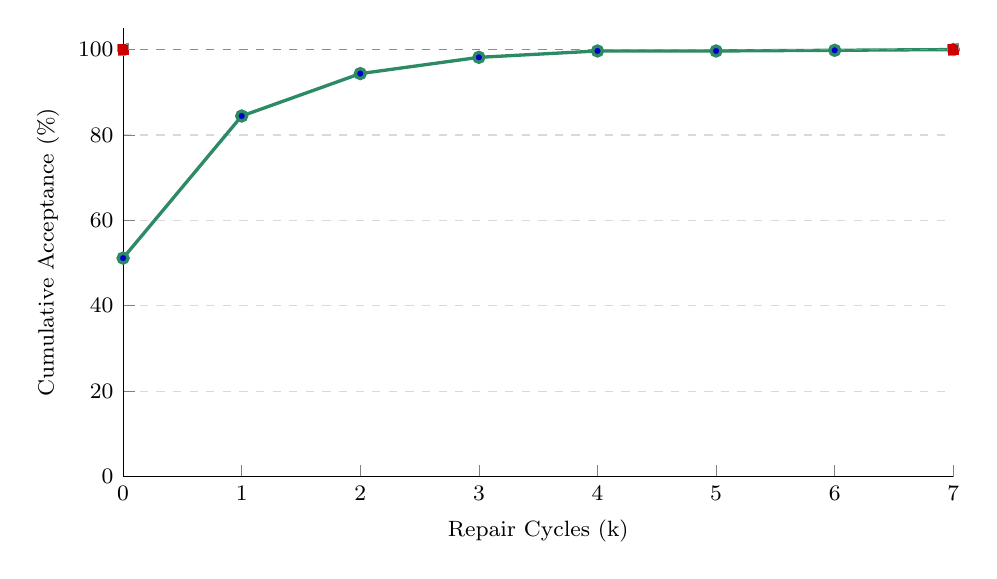
\begin{tikzpicture}
\begin{axis}[
    width=\columnwidth,
    height=0.60\columnwidth,
    xmin=0,
    xmax=7,
    ymin=0,
    ymax=105,
    xlabel={Repair Cycles (k)},
    ylabel={Cumulative Acceptance (\%)},
    xtick={0,1,2,3,4,5,6,7},
    ymajorgrids=true,
    xmajorgrids=false,
    grid style={dashed,gray!30},
    axis lines*=left,
    tick label style={font=\footnotesize},
    label style={font=\footnotesize},
]
\addplot+[pipelineColor, very thick, mark=*, mark size=1.8pt] coordinates {
    (0,51.16)
    (1,84.44)
    (2,94.37)
    (3,98.18)
    (4,99.67)
    (5,99.67)
    (6,99.83)
    (7,100.00)
};
\addplot+[black!45, dashed, thin] coordinates {(0,100) (7,100)};
\end{axis}
\end{tikzpicture}
